\chapter{Introduction}
% \todo{parcours math + grandir musique + gravure musicale avec foot note}
% \todo{analogie avec la free party heretik}

Ma découverte du monde des \textit{shaders} a été un véritable tournant dans mon parcours. Préalablement à ma formation ATI, j'ai eu l'opportunité d'acquérir une expérience précieuse en tant que développeur au sein du département R\&D de Xilam Animation.

C'est grâce à mon mentor de l'époque, Antoine Boellinger, responsable du \textit{pipeline} et ancien d'ATI, que j'ai pris conscience de l'existence même des \textit{shaders}. Cette révélation a été pour moi comme un choc électrique : la possibilité de créer des images à partir des mathématiques m'a semblé magique et m'a profondément intrigué. Dès lors, j'ai ressenti le besoin d'approfondir mes connaissances dans ce domaine.

C'est au cours de la formation ATI que j'ai également eu l'opportunité d'assister à une conférence du Cookie Collective à la Gaîté Lyrique, expérience qui a été tout aussi marquante. Lors de cet événement, j'ai été impressionné par la capacité des artistes à improviser des visuels projetés sur grand écran, ainsi que par l'utilisation de langages ésotériques pour produire de la musique. Ce spectacle a éveillé en moi le désir de pouvoir un jour les imiter.

Depuis maintenant un peu plus d'un an, j'ai eu la chance d'assister à des ateliers animés par z0rg au \textit{hackerspace}\footnote{Un \textit{hackerspace} est un espace physique où des passionnés de technologie, de programmation informatique et de création collaborative se réunissent pour travailler sur des projets, échanger des connaissances et partager des ressources.} le Fuz. Grâce à son approche pédagogique qui va droit au but, j'ai pu acquérir une grande partie de mes connaissances actuelles sur les \textit{shaders}. Ces ateliers m'ont également permis de découvrir une communauté particulièrement généreuse, tant sur le plan humain que sur le plan du partage des connaissances, et m'ont sensibilisé à l'esprit de l'\textit{open source}\footnote{L'esprit \textit{open source} se réfère à une approche collaborative et transparente du développement de logiciels et de technologies, basée sur le partage libre et ouvert du code source. Les projets \textit{open source} permettent à quiconque d'accéder, d'étudier, de modifier et de redistribuer le code source d'un logiciel, favorisant ainsi la collaboration et l'innovation collective.}.

\begin{figure}[h]
  \begin{minipage}[b]{0.45\linewidth}
    \centering
    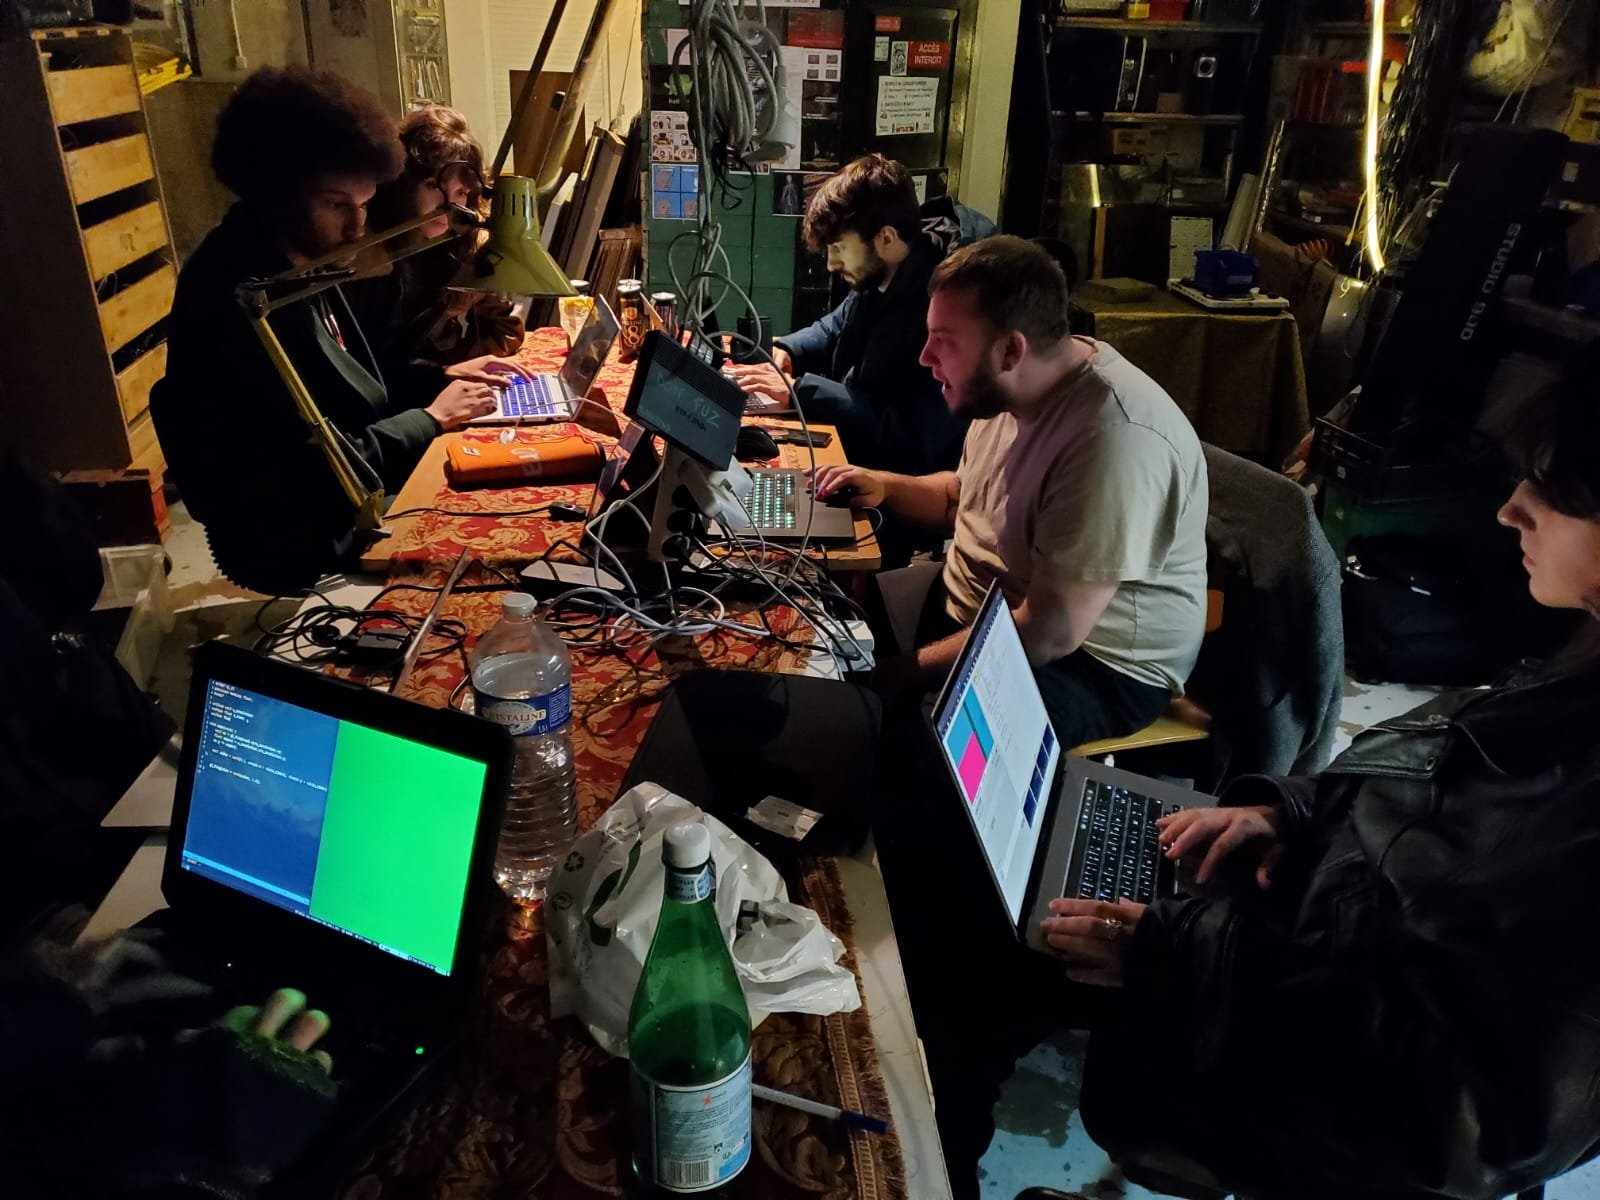
\includegraphics[width=\linewidth]{images/introduction/intro04.jpg}
    \caption{Ateliers \textit{creative coding} au Fuz (photo Léon Denise)}
    \label{intro04}
  \end{minipage}
  \hspace{0.1\linewidth} % Espace horizontal pour la gouttière
  \begin{minipage}[b]{0.45\linewidth}
    \centering
    \includegraphics[width=\linewidth]{images/introduction/intro07.png}
    \caption{Performance son / visuels (photo Émilie Corne)}
    \label{intro07}
  \end{minipage}
\end{figure}

À noter aussi qu'une certaine frustration a marqué mon parcours : le sentiment de saturation lié à l'utilisation intensive de logiciels. Pour répondre à cette frustration, j'ai décidé de m'éloigner autant que possible de ces outils, dans une volonté affirmée de sortir de ma zone de confort.

Cette expérience avec le Cookie Collective a été source d'inspiration pour moi et a réaffirmé l'importance de la liberté créative et du pouvoir du collectif. Elle a ravivé en moi l'espoir en un art novateur, capable de dépasser les limites du « cinéma » tel que nous le connaissons aujourd'hui, et d'explorer de nouvelles voies d'expression artistique. L'esprit de communauté et l'organisation autonome de ce collectif m'ont rappelé les mouvements de \textit{free parties}\footnote{Les \textit{free parties} sont des événements musicaux et culturels autonomes, souvent organisés de manière clandestine et sans autorisation officielle, caractérisés par une programmation musicale centrée sur la musique électronique \textit{underground}. Ces événements se déroulent généralement dans des lieux inhabituels ou alternatifs, tels que des entrepôts abandonnés, des champs, des forêts ou des \textit{squats}.} des années 90 qui ont eu une influence profonde sur la culture et l'esthétique numériques contemporaines.

En assistant aux performances, j'ai constaté que l'interaction entre le \textit{livecoder} de \textit{shaders} et celui de musique était artificielle. Habituellement, c'est le \textit{livecoder} des \textit{shaders} qui ajuste ses variables en fonction du son qu'il entend, permettant ainsi au visuel de suivre le rythme. Bien que cela puisse duper le public, cette observation m'a incité à rechercher un moyen d'obtenir une interaction authentique entre le son et le visuel. C'est précisément le sujet principal abordé dans ce mémoire.

Dans la première partie, je revisiterai les origines de la \textit{demoscene}, en adoptant un angle plus historique que technique. Cette démarche répond à un double objectif : enrichir ma culture personnelle et mieux comprendre cet univers pour m'y intégrer pleinement. 

La deuxième partie, précédée d'un bref rappel sur le \textit{pipeline} graphique, constitue une sorte de tutoriel visant à présenter les techniques essentielles du \textit{livecoding}. Pour des raisons de lisibilité, j'ai opté pour une décomposition en deux sections. La première traitera des techniques fondamentales pour écrire des \textit{fragment shaders} en temps réel, tandis que la seconde explorera des techniques plus avancées mais optionnelles.

Conscient que certains de mes camarades de promotion sont passionnés par le développement et la manipulation des \textit{shaders} sans nécessairement maîtriser la logique mathématique sous-jacente, j'ai cherché à rendre ces concepts accessibles et didactiques. J'espère ainsi susciter leur intérêt pour la programmation des \textit{shaders}.

Enfin, la dernière partie de ce mémoire sera consacrée à mes expérimentations, mettant en lumière certains langages spécifiques au \textit{livecoding} musical, notamment FoxDot et Orca. Ces solutions se sont avérées parfaitement adaptées à mes besoins, car FoxDot offre une expérience proche de la notation musicale traditionnelle, en rapport avec mon expérience en gravure musicale\footnote{La gravure musicale est le processus de notation ou de transcription de la musique dans un format numérique à l'aide de logiciels spécialisés. Cette pratique consiste à représenter les éléments musicaux tels que les notes, les rythmes, les indications de tempo, les dynamiques et d'autres instructions d'interprétation de manière visuelle et compréhensible pour les musiciens. Les principales solutions logicielles de gravure musicale comprennent des programmes tels que Finale, MuseScore et LilyPond (ma solution privilégiée).}, tandis qu'Orca m'a séduit par sa syntaxe originale et sa créativité graphique.

Après avoir exploré en détail la structure d'un fichier MIDI (consultable en annexe), la fin de cette dernière partie sera consacrée à l'introduction d'une solution visant à récupérer les informations MIDI en vue d'animer un \textit{shader}. Cette approche évite l'utilisation de logiciels tiers pour se rapprocher d'un \textit{pipeline} de développement purement basé sur le code.

Il me semblait aussi important de souligner que mon intention première était d'inclure des chapitres dédiés à l'\textit{algorave} et à la musique algorithmique. Cependant, en raison d'une contrainte de temps et d'une surestimation de mes capacités, j'ai été contraint d'abandonner ces sujets.

\newpage


\begin{figure}[htbp]
  \begin{minipage}[b]{0.45\linewidth}
    \centering
    \includegraphics[width=\linewidth]{images/introduction/intro06.png}
    \caption{Performance musique/\textit{shaders} (photo Émilie Corne)}
    \label{intro06}
  \end{minipage}
  \hspace{0.1\linewidth} % Espace horizontal pour la gouttière
  \begin{minipage}[b]{0.45\linewidth}
    \centering
    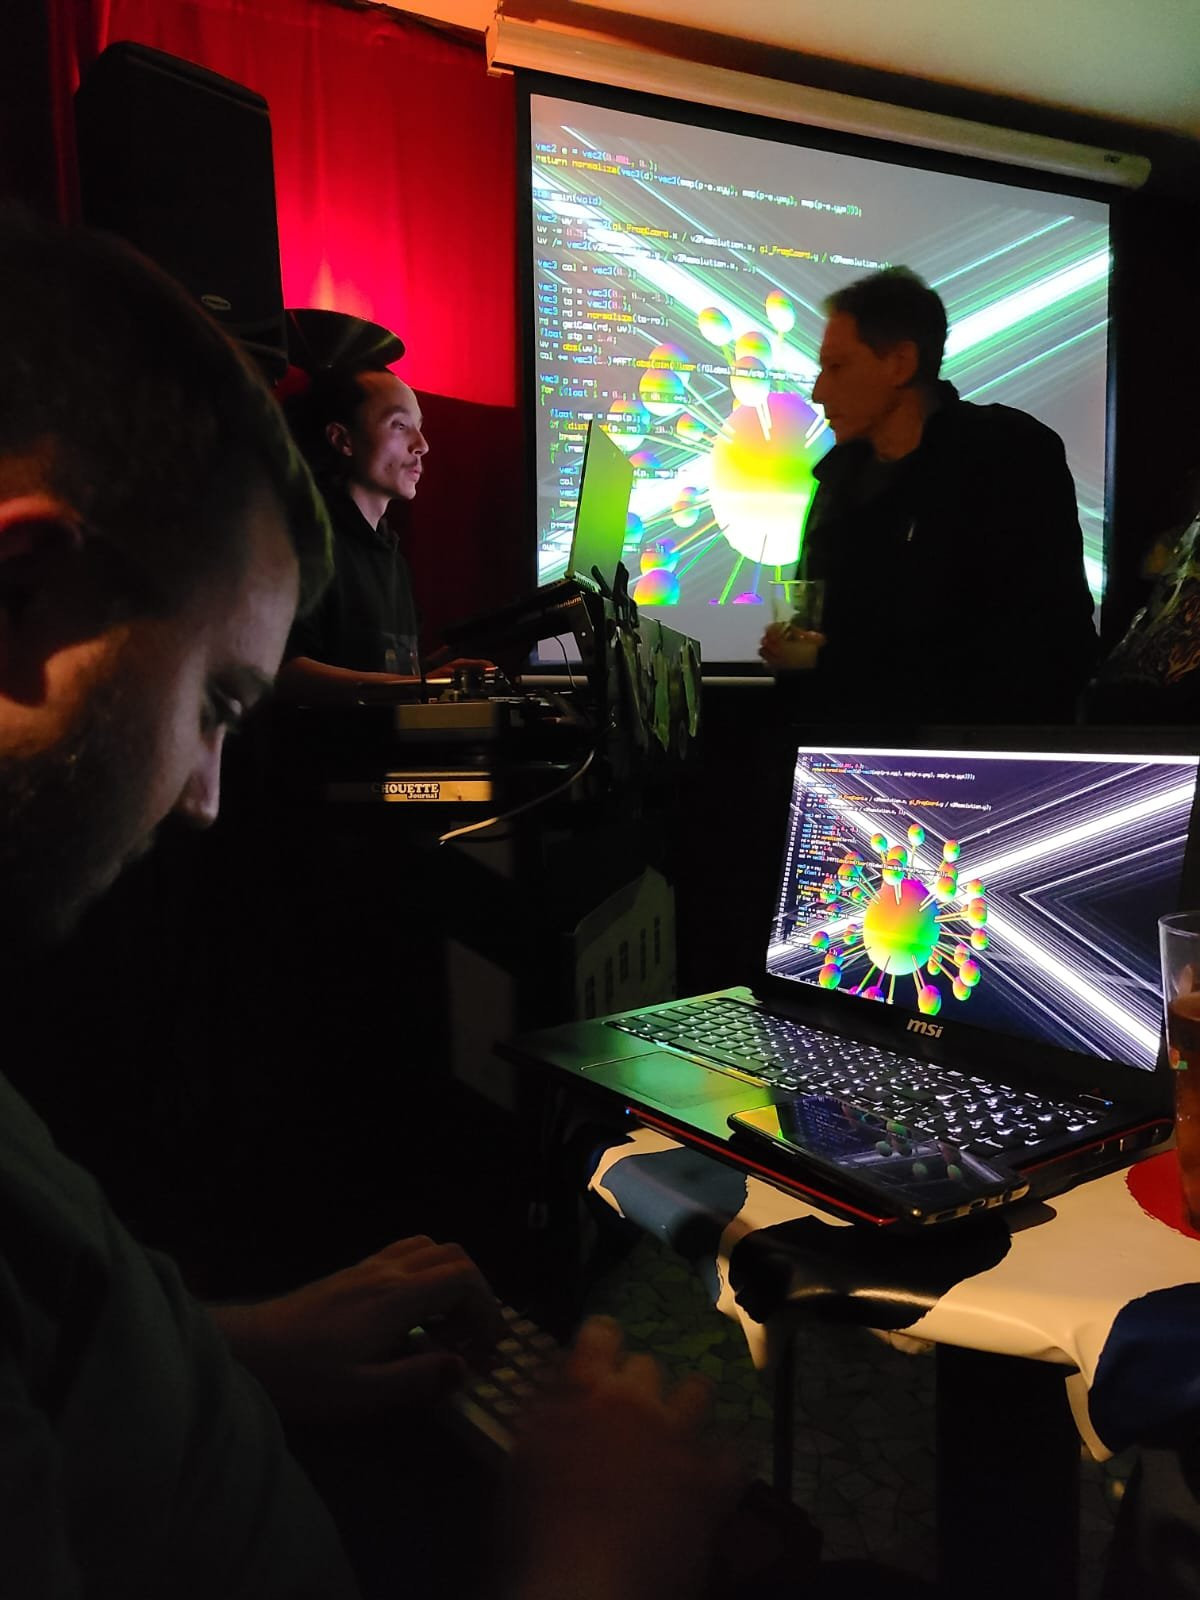
\includegraphics[width=\linewidth]{images/introduction/intro02.jpg}
    \caption{Performance musique/\textit{shaders} au bar la Chair de Poule (photo Léon Denise)}
    \label{intro02}
  \end{minipage}
\end{figure}
